\RequirePackage{ifpdf}
\documentclass[12pt]{JHEP3}

\usepackage{url}
%\usepackage[dvips]{epsfig}
\usepackage{graphicx}

\def\vec#1{\ifmmode
\mathchoice{\mbox{\boldmath$\displaystyle\bf#1$}}
{\mbox{\boldmath$\textstyle\bf#1$}}
{\mbox{\boldmath$\scriptstyle\bf#1$}}
{\mbox{\boldmath$\scriptscriptstyle\bf#1$}}\else
{\mbox{\boldmath$\bf#1$}}\fi}

\newcommand{\Pois}{{\ensuremath{\rm Pois}}}


\author{Usama Hussain$^{a}$\\
$^{a}$ New York University Abu Dhabi
}

\date{April 16, 2014}

\title{Your Title here}

\abstract{Abstract here}

\begin{document}


\section{Introduction}

\begin{equation}
e^{i\pi}+1=0
\label{eq:myequation}
\end{equation}

See Equation~\ref{eq:my equation} and my Figure~\ref{fig:myFig}.

\begin{figure}
\center
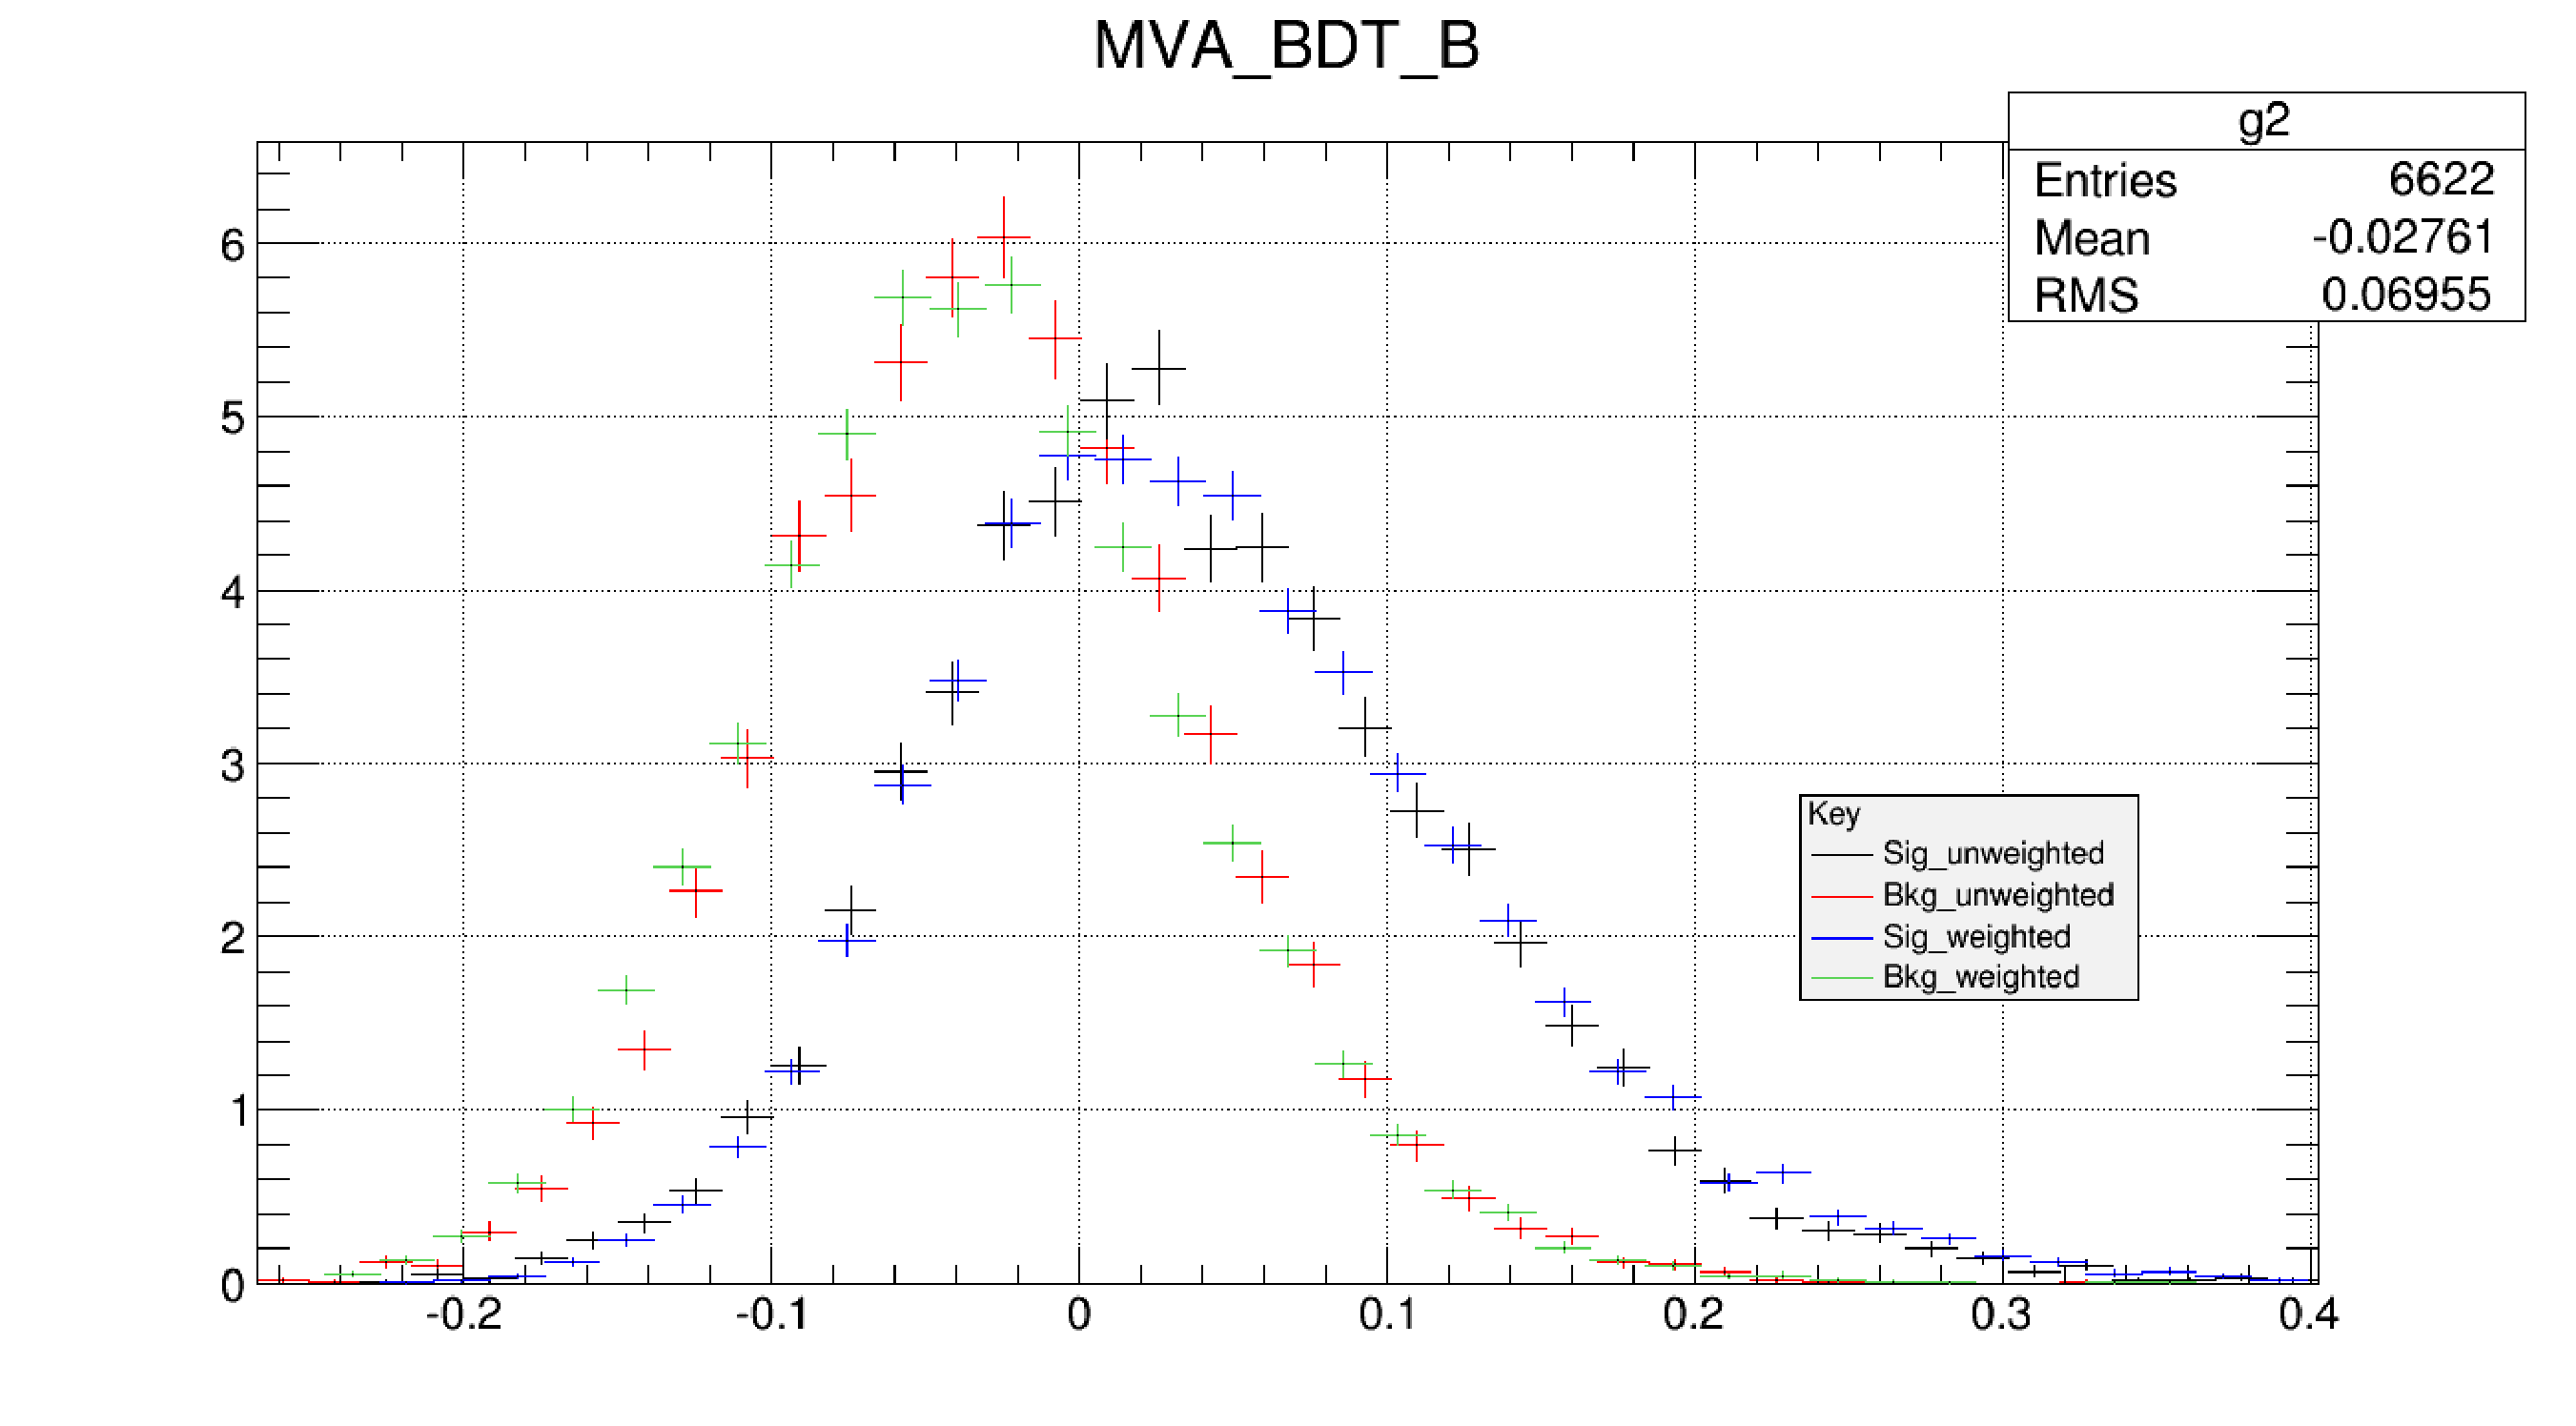
\includegraphics[width=.7\textwidth]{BDT_test_WvUn.pdf}
\caption{Hello}
\label{fig:myFig}
\end{figure}



\section*{Acknowledgements}

Blah
%\bibliographystyle{JHEP}
%\bibliography{fisher}

\end{document}
